\documentclass[class=jsarticle, crop=false, dvipdfmx, fleqn]{standalone}
%% preamble for Numerical-structure-analysis report

\input{/Users/User/Documents/Project/TeX/preamble/mypreamble}

%% titles
\title{先端データ解析論 レポート}
\author{37-196360 \quad 森田涼介}


%% setting for listings
\newtcbinputlisting[auto counter]{\reportlisting}[3][]{%
	listing file = {#3},
	listing options = {language=python, style=tcblatex, numbers=left, numberstyle=\tiny},
	listing only,
	breakable,
	toprule at break = 0mm,
	bottomrule at break = 0mm,
	left = 6mm,
	sharp corners,
	drop shadow,
	title = Listings \thetcbcounter : \texttt{#2},
	label = #1,
	}



%% title format
\usepackage{titlesec}
\titleformat{\section}{\LARGE}{宿題\thesection}{0zw}{}
\newcommand{\sectionbreak}{\clearpage}
\titleformat{\subsection}{\Large}{\Alph{subsection})}{0zw}{}

\begin{document}
\section{}

ガウスカーネルモデルに対して,最小二乗確率的分類を実装する。
\begin{align}
    & q\qty(y\ |\ \bm{x};\ \bm{\theta}^{(y)})
        = \sum_{j:y_j = y} \theta_j^{(y)} K(\bm{x},\ \bm{x}_j) \\
    & K(\bm{x},\ \bm{c}) = \exp(- \frac{||\bm{x} - \bm{c}||^2}{2 h^2})
\end{align}
二乗誤差は次のようになる。
\begin{align}
    J_y (\bm{\theta}_y)
        & = \frac{1}{2} \int \qty(q(y|\bm{x};\ \bm{\theta}_y) - p(y\ |\ \bm{x}))^2 p(\bm{x}) \dd\bm{x} \\
        & =
            \frac{1}{2} \int \qty(q(y|\bm{x};\ \bm{\theta}_y))^2 p(\bm{x}) \dd\bm{x}
            - \int q(y|\bm{x};\ \bm{\theta}_y) p(y|\bm{x}) p(\bm{x}) \dd\bm{x}
            + \frac{1}{2} \int p(y|\bm{x})^2 p(\bm{x}) \dd\bm{x}
\end{align}
これを標本近似することを考える。
第一項は,
\begin{equation}
    \frac{1}{2} \int \qty(q(y|\bm{x};\ \bm{\theta}_y))^2 p(\bm{x}) \dd\bm{x}
        \ \rightarrow\ 
        \frac{1}{2} \cdot \frac{1}{n} \sum_{i=1}^{n} q(y|\bm{x}_i;\ \bm{\theta}_y)^2
\end{equation}
第二項は,
\begin{align}
    \int q(y|\bm{x};\ \bm{\theta}_y) p(y|\bm{x}) p(\bm{x}) \dd\bm{x}
        & = \int q(y|\bm{x};\ \bm{\theta}_y) p(y) p(\bm{x}|y) \dd\bm{x} \\
        & = p(y) \int q(y|\bm{x};\ \bm{\theta}_y) p(\bm{x}|y) \dd\bm{x} \\
        & \rightarrow \frac{n_y}{n} \cdot \frac{1}{n_y} \sum_{i:y_i=y} q(y|\bm{x}_i;\ \bm{\theta}_y) \\
        & = \frac{1}{n} \sum_{i:y_i=y} q(y|\bm{x}_i;\ \bm{\theta}_y)
\end{align}
第三項は定数なので無視できる。
以上にL2正則化項を加えると,
二乗誤差は,
\begin{align}
    \hat{J}_y (\bm{\theta}_y)
        & =
            \frac{1}{2n} \sum_{i=1}^{n} q(y|\bm{x}_i;\ \bm{\theta}_y)^2
            - \frac{1}{n} \sum_{i:y_i=y} q(y|\bm{x}_i;\ \bm{\theta}_y)
            + \frac{\lambda}{2n} ||\bm{\theta}_y||^2 \\
        & = \frac{1}{n} \qty(
            \frac{1}{2} \sum_{i=1}^{n} q(y|\bm{x}_i;\ \bm{\theta}_y)^2
            - \sum_{i:y_i=y} q(y|\bm{x}_i;\ \bm{\theta}_y)
            + \frac{\lambda}{2} ||\bm{\theta}_y||^2
            )
\end{align}
と表せる。

いま,ガウスカーネルモデルを考えると,
カーネル行列
\begin{equation}
    \bm{K} =
        \begin{bmatrix}
            K(\bm{x}_1,\ \bm{x}_1) & \cdots & K(\bm{x}_1,\ \bm{x}_n) \\
            \vdots & \ddots & \vdots \\
            K(\bm{x}_n,\ \bm{x}_1) & \cdots & K(\bm{x}_n,\ \bm{x}_n)
        \end{bmatrix}
\end{equation}
を用いれば,二乗誤差は次のように表せる。
\begin{equation}
    \hat{J}_y (\bm{\theta}_y)
        = \frac{1}{n} \qty{
            \frac{1}{2} \bm{\theta}_y^\mathrm{T} \bm{K}^2 \bm{\theta}_y - \bm{\theta}_y^\mathrm{T} \bm{K} \bm{\pi}_y + \frac{\lambda}{2} ||\bm{\theta}_y||^2
            }
\end{equation}
ここで,\(\bm{K}\)は対称行列であることを利用した。
また,
\begin{equation}
    \pi_{y, i} =
        \begin{cases}
            1 & (y_i = y) \\
            0 & (y_i \neq y)
        \end{cases}
\end{equation}
である。
\(\bm{\theta}_y\)による偏微分は,
\begin{align}
    \pdv{\hat{J}_y}{\bm{\theta}_y}
        & = \frac{1}{n} \qty{
            \bm{K}^2 \bm{\theta}_y - \bm{K} \bm{\pi}_y + \lambda \bm{\theta}_y
            } \\
        & = \frac{1}{n} \qty{
            \qty(\bm{K}^2 + \lambda \bm{I}) \bm{\theta}_y - \bm{K} \bm{\pi}_y
            }
\end{align}
これを\(\bm{0}\)にするような\(\bm{\theta}_y\)は,
\begin{equation}
    \hat{\bm{\theta}}_y = \qty(\bm{K}^2 + \lambda \bm{I})^{-1} \bm{K} \bm{\pi}_y
\end{equation}
となる。
プログラムでは,この式を用いてパラメータを求める。

バンド幅\(h = 2.0\),L2正則化パラメータ\(\lambda = 0.0001\)に対する結果を,
以下の図\ref{fig:result}に示す。
なお,プログラムは\pageref{listing:assignment1}ページのListing \ref{listing:assignment1}に示した。

\begin{figure}[H]
    \centering
    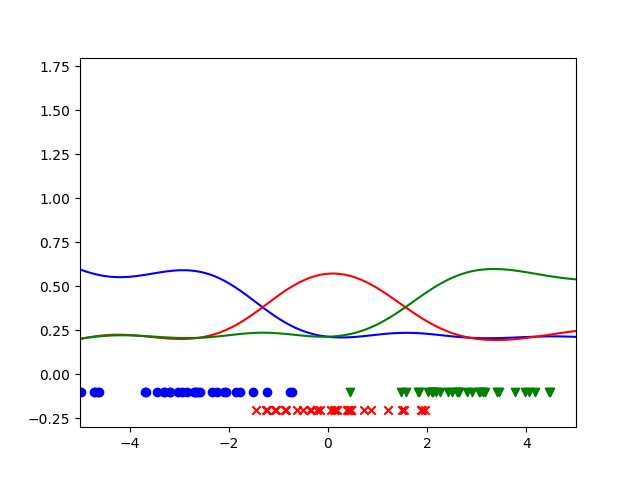
\includegraphics[clip, width=12cm]{../figures/assignment1_result}
    \caption{結果}
    \label{fig:result}
\end{figure}


\end{document}
